\section*{Chapter 6}

\subsection*{Exercise 6.1}
If $V$ changes during the episode, then (6.6) only holds approximately; what
would the difference be between the two sides? Let $V_t$ denote the array of state values
used at time $t$ in the TD error (6.5) and in the TD update (6.2). Redo the derivation
above to determine the additional amount that must be added to the sum of TD errors
in order to equal the Monte Carlo error. 

\subsubsection*{Solution:}

\begin{align*}
G_t - V(S_t) &= R_{t+1} + \gamma G_{t+1} - V_t(S_t) + \gamma V_{t}(S_{t+1}) - \gamma V_{t}(S_{t+1}) \\
&= \delta_t + \gamma G_{t+1} - \gamma V_t(S_{t+1}) \\
&= \delta_t + \gamma R_{t+2} + \gamma^2 G_{t+2} - \gamma V_{t}(S_{t+1}) \\
&= \delta_t + \gamma (R_{t+2} + \gamma V_{t+1}(S_{t+2}) - V_{t+1}(S_{t+1}) - \gamma V_{t+1}(S_{t+2}) + V_{t+1}(S_{t+1}))\\
& \quad + \gamma^2 G_{t+2} - \gamma V_{t}(S_{t+1}) \\
&= \delta_t + \gamma \delta_{t+1} - \gamma^2 V_{t+1}(S_{t+2}) + \gamma V_{t+1}(S_{t+1}) + \gamma^2 G_{t+2} - \gamma V_{t}(S_{t+1})\\
& \dots \\
&= \sum_{k=t}^{T-1} \gamma^{k-t} \delta_k + \sum_{k=t+1}^{T-1} \gamma^{k-t } \left[V_{k}(S_{k}) - V_{k-1}(S_{k}) \right]
\end{align*}


\subsection*{Exercise 6.2}
This is an exercise to help develop your intuition about why TD methods
are often more efficient than Monte Carlo methods. Consider the driving home example
and how it is addressed by TD and Monte Carlo methods. Can you imagine a scenario
in which a TD update would be better on average than a Monte Carlo update? Give
an example scenario — a description of past experience and a current state—in which
you would expect the TD update to be better. Here's a hint: Suppose you have lots
of experience driving home from work. Then you move to a new building and a new
parking lot (but you still enter the highway at the same place). Now you are starting
to learn predictions for the new building. Can you see why TD updates are likely to be
much better, at least initially, in this case? Might the same sort of thing happen in the
original scenario?

\subsubsection*{Solution:}

In the example scenario, after moving to a new building and a new parking lot, the agent still enters the highway at the same place. 
The agent has a lot of experience driving home from work, so it has a good estimate of the value of the state of entering the highway.
However, the agent has no experience with the new building and parking lot, so the Monte Carlo update would require the agent to drive
home from work many times to get a good estimate of the value of the state of the new building and parking lot. On the other hand, the
TD update would only require the agent to drive home from work once (or twice) to get a good estimate of the value of the state of the parking lot
and new building. Therefore, the TD update would be better in this case.


\subsection*{Exercise 6.3}
From the results shown in the left graph of the random walk example it
appears that the first episode results in a change in only V(A). What does this tell you
about what happened on the first episode? Why was only the estimate for this one state
changed? By exactly how much was it changed? 

\subsubsection*{Solution:}
It tells us that the first episode ended on the left side of the random walk.
The update equation:
\[
V(S_t) \leftarrow V(S_t) + \alpha \left[R_{t+1} + \gamma V(S_{t+1}) - V(S_t)\right]
\]

$\gamma = 1$, $\alpha = 0.1$, $V(A) = 0.5$, $V(B) = 0.5$, $V(C) = 0.5$, $V(D) = 0.5$, $V(E) = 0.5$.

While the agent receives a reward of 0, the following happens:

\[
V(S_t) \leftarrow 0.5 + 0.1 \left[0 + 1 \cdot 0.5 - 0.5\right] = 0.5
\]

After the agent chose to go left at state $A$, with $V(\text{terminal state}) = 0$:
\[
V(A) \leftarrow 0.5 + 0.1 \left[0 + 1 \cdot 0 - 0.5\right] = 0.45
\]


\subsection*{Exercise 6.4}
The specific results shown in the right graph of the random walk example
are dependent on the value of the step-size parameter, $\alpha$. Do you think the conclusions
about which algorithm is better would be affected if a wider range of $\alpha$ values were used?
Is there a different, fixed value of $\alpha$ at which either algorithm would have performed
significantly better than shown? Why or why not?

\subsubsection*{Solution:}
Using different values of $\alpha$ would not affect the conclusions about which algorithm is better.
If $\alpha$ would be smaller, the algorithms would converge slower, but would approximate the true value function better.
If $\alpha$ would be larger, the algorithms would converge faster, but would approximate the true value function worse, as we are more dependent on the more recently observed rewards.

\subsection*{*Exercise 6.5}
In the right graph of the random walk example, the RMS error of the
TD method seems to go down and then up again, particularly at high $\alpha$'s. What could
have caused this? Do you think this always occurs, or might it be a function of how the
approximate value function was initialized? 

\subsubsection*{Solution:}
The increase in RMS error for TD at high $\alpha$ values is due to instability and overshooting caused by 
large step sizes, leading to divergence from the true values. While initialization can affect early learning dynamics,
it does not prevent this instability at high $\alpha$.

\subsection*{Exercise 6.6}
In Example 6.2 we stated that the true values for the random walk example
are $\frac{1}{6}, \frac{2}{6}, \frac{3}{6}, \frac{4}{6}$, and $\frac{5}{6}$ for states A through E. Describe at least two different ways that
these could have been computed. Which would you guess we actually used? Why?

\subsubsection*{Solution:}

We could write this as a system of linear equations:
\[
\begin{bmatrix}
    0 & 0.5 & 0 & 0 & 0 \\
    0.5 & 0 & 0.5 & 0 & 0 \\
    0 & 0.5 & 0 & 0.5 & 0 \\
    0 & 0 & 0.5 & 0 & 0.5 \\
    0 & 0 & 0 & 0.5 & 0 
\end{bmatrix}
\begin{bmatrix}
    V(A) \\
    V(B) \\
    V(C) \\
    V(D) \\
    V(E) 
\end{bmatrix}
+
\begin{bmatrix}
    0 \\
    0 \\
    0 \\
    0 \\
    0.5
\end{bmatrix}
=
\begin{bmatrix}
    V(A) \\
    V(B) \\
    V(C) \\
    V(D) \\
    V(E) 
\end{bmatrix}
\]

\[
    \begin{bmatrix}
        -1 & 0.5 & 0 & 0 & 0 \\
        0.5 & -1 & 0.5 & 0 & 0 \\
        0 & 0.5 & -1 & 0.5 & 0 \\
        0 & 0 & 0.5 & -1 & 0.5 \\
        0 & 0 & 0 & 0.5 & -1 
    \end{bmatrix}
    \begin{bmatrix}
        V(A) \\
        V(B) \\
        V(C) \\
        V(D) \\
        V(E) 
    \end{bmatrix}
    =
    \begin{bmatrix}
        0 \\
        0 \\
        0 \\
        0 \\
        -0.5
    \end{bmatrix}
\]

\[
    \begin{bmatrix}
        V(A) \\
        V(B) \\
        V(C) \\
        V(D) \\
        V(E) 
    \end{bmatrix}
    =
    \begin{bmatrix}
        1/6 \\
        2/6 \\
        3/6 \\
        4/6 \\
        5/6
    \end{bmatrix}
\]

Or we could also solve this problem with the dynamic programming approach. I think this way used, as it is relevant to the context of the book.

\subsection*{*Exercise 6.7}
Design an off-policy version of the TD(0) update that can be used with
arbitrary target policy $\pi$ and covering behavior policy $b$, using at each step $t$ the importance
sampling ratio $\rho_{t:t}$ (5.3).

\subsubsection*{Solution:}

\begin{align*}
    V(S_t) &= \mathbb{E}_\pi[G_t \mid S_t = s] \\
    &= \sum_{a} \pi(a \mid s) \sum_{s', r} p(s', r \mid s, a) \left[ r + \gamma V(s') \right] = \\
    &= \sum_{a} b(a \mid s) \sum_{s', r} p(s', r \mid s, a) \frac{\pi(a \mid s)}{b(a \mid s)} \left[ r + \gamma V(s') \right] \left[ r' + \gamma V(s'') \right] \\
    &= \mathbb{E}_b[\rho_{t:t} G_t \mid S_t = s] = \mathbb{E}_b[\rho_{t:t} (R_{t+1} + \gamma V(S_{t+1})) \mid S_t = s]
\end{align*}


\[
V(S_t) \leftarrow V(S_t) + \alpha  \left[ \rho_{t:t}(R_{t+1} + \gamma V(S_{t+1})) - V(S_t) \right]
\]

\subsection*{Exercise 6.8}
Show that an action-value version of (6.6) holds for the action-value form
of the TD error  $\delta_t = R_{t+1} + \gamma Q(S_{t+1}, A_{t+1}) - Q(S_t, A_t)$, again assuming that the values
don't change from step to step. 

\subsubsection*{Solution:}

\begin{align*}
    G_t - Q(S_t, A_t) &= R_{t+1} + \gamma G_{t+1} - Q(S_t, A_t) + \gamma Q(S_{t+1}, A_{t+1}) - \gamma Q(S_{t+1}, A_{t+1}) \\
    &= \delta_t + \gamma (G_{t+1} - Q(S_{t+1}, A_{t+1})) \\
    &= \delta_t + \gamma \delta_{t+1} + \gamma^2 (G_{t+2} - Q(S_{t+1}, A_{t+2})) \\
    &= \delta_t + \gamma \delta_{t+1} + \gamma^2 \delta_{t+2} + \cdots + \gamma^{T-t-1} \delta_{T-1} + \gamma^{T-t} (G_T - Q(S_{T}, A_{T})) \\
    &= \delta_t + \gamma \delta_{t+1} + \gamma^2 \delta_{t+2} + \cdots + \gamma^{T-t-1} \delta_{T-1} + \gamma^{T-t} (0 - 0) \\
    &= \sum_{k=t}^{T-1} \gamma^{k-t} \delta_k.
\end{align*}


\subsection*{Exercise 6.9: Windy Gridworld with King's Moves (programming)}
Re-solve the windy gridworld assuming eight possible actions, including the diagonal moves, rather than four.
How much better can you do with the extra actions? Can you do even better by including
a ninth action that causes no movement at all other than that caused by the wind?

\subsubsection*{Solution:}
See the notebook.
\begin{figure}[H]
    \centering
    \begin{minipage}[b]{0.47\textwidth}
      \centering
      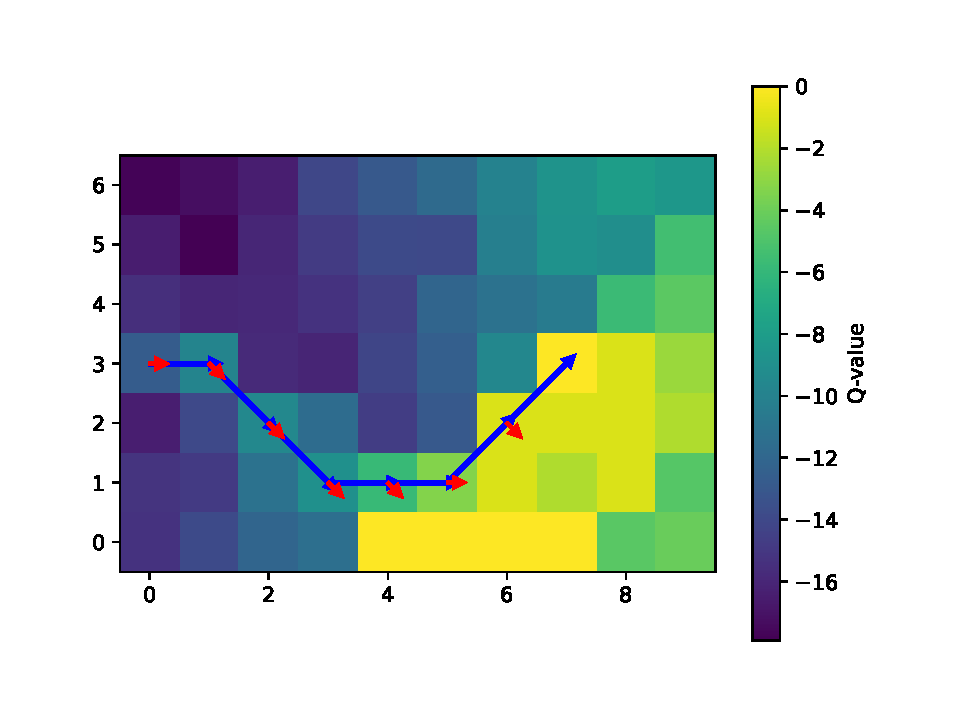
\includegraphics[width=\textwidth]{chapters_latex/figures/ex_06_09_king_moves.pdf}
      \captionsetup{labelformat=empty}
      \caption{King's Moves}
      
    \end{minipage}
    \hspace{0.04\textwidth} % Adjusts the horizontal space between images
    \begin{minipage}[b]{0.47\textwidth}
        \centering
        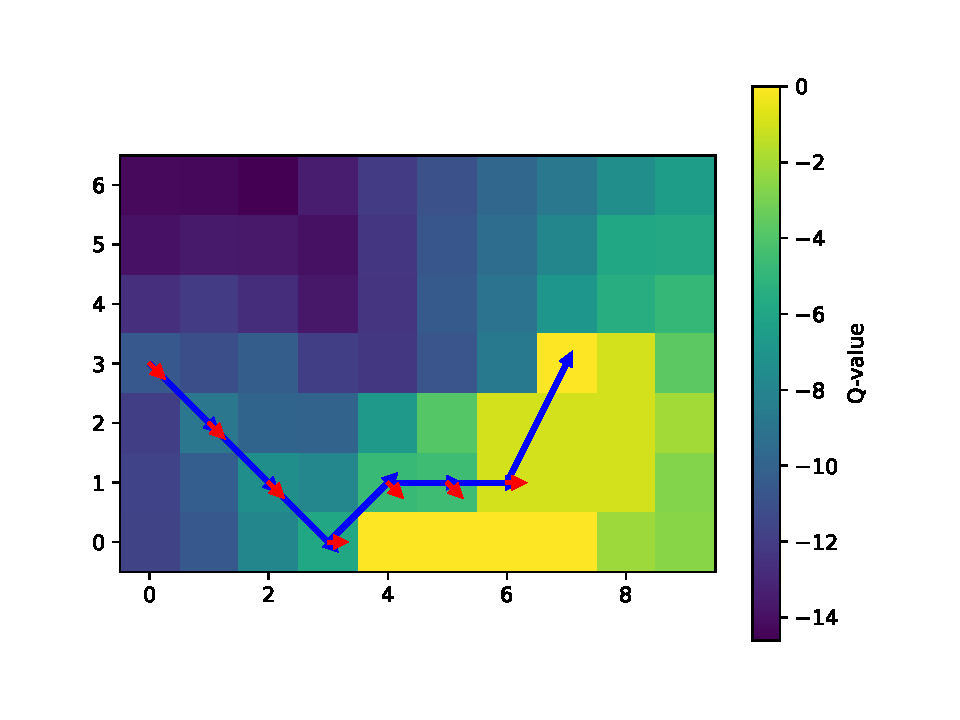
\includegraphics[width=\textwidth]{chapters_latex/figures/ex_06_09_king_moves_plus_zero.pdf}
        \captionsetup{labelformat=empty}
        \caption{King's Moves and Zero Action}
    \end{minipage}
  \end{figure}

\subsection*{Exercise 6.10: Stochastic Wind (programming)}
Re-solve the windy gridworld task with
King's moves, assuming that the effect of the wind, if there is any, is stochastic, sometimes
varying by 1 from the mean values given for each column. That is, a third of the time
you move exactly according to these values, as in the previous exercise, but also a third
of the time you move one cell above that, and another third of the time you move one
cell below that. For example, if you are one cell to the right of the goal and you move
left , then one-third of the time you move one cell above the goal, one-third of the time
you move two cells above the goal, and one-third of the time you move to the goal.

\subsubsection*{Solution:}
See the notebook.
\begin{figure}[H]
    \centering
    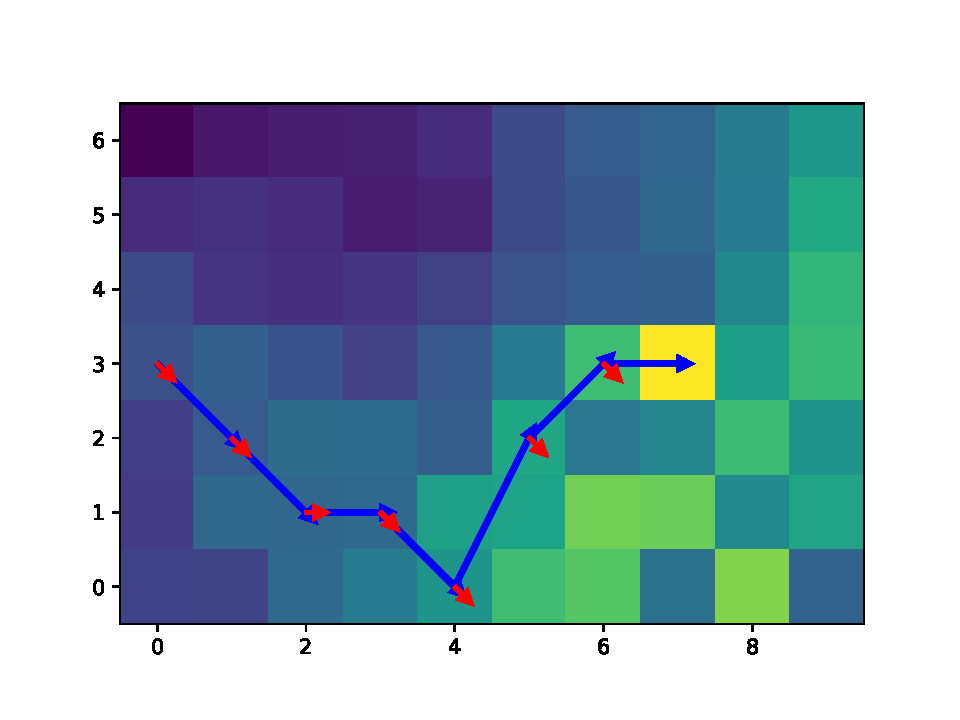
\includegraphics[width=0.65\textwidth]{chapters_latex/figures/ex_06_10.pdf}
    \captionsetup{labelformat=empty}
    \caption{King's Moves and Stochastic Wind}
\end{figure}

The average number of steps to reach the goal is 13.449 in my implementation, this could be improved by tuning the hyperparameters ($\varepsilon$, $\alpha$) and the number of episodes.

\subsection*{Exercise 6.11}
Why is Q-learning considered an off-policy control method?

\subsubsection*{Solution:}
Q-learning is an off-policy method because it learns the optimal policy independently of the
agent's current behavior policy by updating Q-values based on the maximum possible future reward, not the action actually taken.

\subsection*{Exercise 6.12}
Suppose action selection is greedy. Is Q-learning then exactly the same
algorithm as Sarsa? Will they make exactly the same action selections and weight
updates?

\subsubsection*{Solution:}
If action selection is greedy for both Q-learning and SARSA, is can be said that they are the same algorithm. 

The update for Q-learning:
\[
Q(s, a) \leftarrow Q(s, a) + \alpha \left( r + \gamma \max_{a'} Q(s', a') - Q(s, a) \right)
\]

The update for SARSA:
\[
Q(s, a) \leftarrow Q(s, a) + \alpha \left( r + \gamma Q(s', a') - Q(s, a) \right)
\]
Where $Q(s', a') = \max_{a'} Q(s', a')$

These are the same, so the updates are equal for the same $s$ and $a$.

Since both algorithms have the same policy, they will make the same action selections too.


\subsection*{*Exercise 6.13}
What are the update equations for Double Expected Sarsa with an
$\varepsilon$-greedy target policy?

\subsubsection*{Solution:}
The Expected SARSA update equation is:
\[
    Q(S_t, A_t) \leftarrow Q(S_t, A_t) + \alpha \left[ R_{t+1} + \gamma \sum_{a} \pi(a \mid S_{t+1}) Q(S_{t+1}, a) - Q(S_t, A_t) \right]
\]

Double Expected Sarsa with an
$\varepsilon$-greedy target policy update:

\[
    Q_1(S_t, A_t) \leftarrow Q_1(S_t, A_t) + \alpha \left[ R_{t+1} + \gamma \sum_{a} \pi(a \mid S_{t+1}) Q_2(S_{t+1}, a) - Q_1(S_t, A_t) \right]
\]
where
\[
    \sum_{a} \pi(a \mid S_{t+1}) Q_2(S_{t+1}, a) = \frac{\varepsilon}{|A(a)|} \sum_{a} Q_2(S_{t+1}, a) + (1- \varepsilon) \max_{a'} Q_2(S_{t+1}, a')
\]

And the same for $Q_2$, but with the roles of $Q_1$ and $Q_2$ reversed.


\subsection*{Exercise 6.14}
Describe how the task of Jack's Car Rental (Example 4.2) could be
reformulated in terms of afterstates. Why, in terms of this specific task, would such a
reformulation be likely to speed convergence?

\subsubsection*{Solution:}

In Jack's Car Rental problem, an afterstate formulation would involve focusing on the state of cars
at each location immediately after cars are moved but before rentals occur. This approach simplifies
the problem by associating the rewards directly with the afterstate rather than with the specific state-action pairs.

This reformulation speeds up convergence by reducing dimensionality, as fewer values (one per afterstate) need to be 
learned instead of multiple values for each state-action pair. Additionally, it removes action redundancy by collapsing 
multiple state-action pairs into a single afterstate, leading to simpler, more efficient policy learning.